\Chapter{Implementáció}

Ebben a fejezetben igyekszem bemutatni néhány izgalmasabb esetet, amelyek vagy a bonyolultságuk miatt érdekesek vagy számomra rengeteg fejtörést okoztak amire elkészültek.

\subsubsection{Fesztivál keresés}
A fesztiválok megkereséséhez használtam a legkomplexebb folyamatot. Amelyben először a felület felől meg vizsgáljuk, hogy melyik keresési paramétereket adta meg a felhasználó, és csak azokat a paramétereket küldjük el a szerveroldalra, amelyeket megadta. Az x és y koordinátát egy google maps API-n keresztül szerzem meg, ahol beírja a felhasználó a kívánt települést, a rendszer pedig már a településhez tartozó koordinátákkal dolgozik tovább. Ha nem ír be semmit, akkor ezek az értékek üresek maradnak és a helytől való távolságot sem érdemes elküldeni a túloldalra. Amint látható a HttpParams objektumnak csak string típusú változókat lehet átadni, így cast-olni kellett karakterlánccá az értékeket. A dolog érdekessége, hogy a Spring oldalon ki lehet venni más típusként is.
A lekérdezésből visszaérkezett adathalmazt leképezzük a modellnek megfelelő formára és a modellekből készült tömbbel tér vissza a metódus a megjelenítési réteghez.

A metódus egyik paraméterét sem kötelező átadni neki, hisz ez egy lekérdezés, jöhet kevesebb információval is kérés. Ha érkezik dátum érték azt Date formátumra kell konvertálnunk és csak ezután hívhatjuk meg a a FestivalService festsByQuery metódusát.

A festsByQuery metódust implementáltam A FestivalServiceImpl osztályban. A függvény paraméter szignatúrája a következő: \texttt{(String style, boolean isFree, Date begin, Date end, Double posX, Double posY, Double maxFromPos)} a visszatérési értéke egy \texttt{FestivalDTO} lista. A rendszert minden egyes lehetséges kombinációra fel kell készíteni, természetesen lesznek olyan lekérdezések, amelyeket többször is meghívhatóak más paraméterrel. Abból ered ez, hogy az ingyenességet nem boolean változóban tárolom, hanem stílusparaméterként.
Ha nem kapunk stílust akkor az alábbi ágba fut a programunk.

\begin{java}
if (!isFree) {
festivals = datesWithoutStyle(begin, end, posX, posY, 
maxFromPos);
} else {
    festivals = datesWithStyle("free", begin, end, posX, posY,
    maxFromPos);
}
\end{java}

Ha a felhasználó nem pipálta be, hogy ingyenes legyen a kiválasztott fesztivál, akkor lekérdezzük az adatbázisból a megadott dátumok szerinti eredményt.
Természetesen itt is előfordulhat, hogy nem adott meg dátumokat. Mind a négy lehetséges esetben már belenyúlunk az adatbázisba. Ha sem a kezdő, sem a végdátuma nincs megadva az intervallumnak amelybe keresünk, akkor mindent visszaadunk ami jelen pillanatban még nem fejeződött be.

\begin{java}
festivalRepository.findByEndDateAfterOrderByBeginDate
(new Date(begin.getTime() - 1));
\end{java}

A fenti kódot használhatjuk, ha ismerjük az intervallum kezdetét, de a végét nem. Az előző esetben is ezt a kódot kell használni csak a pillanatnyi dátummal meghívva.
A kód a \texttt{CrudRepository} kiterjesztésével létrehozott \texttt{FestivalRepository} interfészt hívja meg amelyben ha bizonyos név konvenciókat betartunk, akkor automatikusan legenerálja a Query-t(lekérdezést) számunkra. De mint látható ez meglehetősen hosszú metódus neveket szül. A függvény az alábbi paraméterrel azokat adja vissza, amelyiket fesztiválokat a megadott pillanattól kezdve még érdemes meglátogatni. A -1 érték azért van ott, mert sajnos megvannak a határai az automatikusan generált lekérdezésnek és a <= relációt tudtam kisajtolni belőle, csak a < jelet, így egy egységgel csökkentem és akkor már azt kapjuk vissza amit szeretnénk a program kezdésének időpontja szerint rendezve.

\begin{java}
findByEndDateAfterAndBeginDateBeforeOrderByBeginDate(
new Date(), new Date(end.getTime() + 1));
\end{java}

Ha csak azt adja meg a felhasználónk, hogy melyik időpontig alkalmas neki, akkor a \texttt{FestivalRepository} fenti függvényét érdemes meghívni a megadott paraméterekkel.
Ugyan ez a függvény lesz jó nekünk arra, ha mindkettő dátum benne van a kérésben. Az első paramétert le kell cserélnünk \texttt{new Date(begin.getTime() - 1)}-re, hiszen itt megvan adva a \texttt{begin} érték is.

Ezek után a visszakapott értékekkel meg kell hívni a \texttt{workWithPositions(festivals, posX, posY, maxFromPos)} függvényt a megadott szignatúrával. Ez a függvény a Haversine formula segítségével megvizsgálja a megadott paraméterek alapján az átadott fesztiválokat. Ha nem kaptunk pozíciót akkor vissza adunk mindent, ha csak pozíciót kaptunk, akkor az 5 km-en belülieket adjuk vissza, ha kapunk távolságot és pozíciót, akkor a pozíciótól megadott távolságon belüli fesztiválokat adja vissza.

Elképzelhető az is, hogy kiválasztotta a felhasználó, hogy ingyenes fesztiválok érdeklik, vagy esetleg stílust adott meg. Előfordulhat az is, hogy mindkettőt megadta a felhasználó. Mindhárom esetben a fesztivál keresés részben megadott kód else ágában lefutó \texttt{datesWithStyle} függvényre lesz szükségünk, ami nagyon hasonlóan fog működni mint a \texttt{datesWithoutStyle} csak a lekérdezés összes ágában össze kell kapcsolni a \texttt{FestivalStyle} táblával és onnan lekérdezni azokat amelyiknek a \texttt{style} mezője tartalmazza az átadott értéket, a további műveletek már nem változnak ugyan azokon a függvényhívásokon kell átesnie a visszakapott listának. A teljesség igénye nélkül nézzünk meg egy ilyen lekérdezést JPQL segítségével.

\begin{java}
@Query("select f from Festival f inner join f.styles stl where 
lower(stl.style) like lower(:myStyle) and f.endDate >= :begin
and f.beginDate <= :end order by f.beginDate")
List<Festival> 
findByBeginDateBeforeAndEndDateAfterAndStyleOrderByBeginDate
(@Param("myStyle")String style, @Param("begin")Date begin, 
@Param("end")Date end);
\end{java}

Láthatóan itt a kezdő és a végdátum is érkezik paraméterben a stílus mellett. A változókat a \texttt{@Param} annotáció segítségével tudjuk átadni a \texttt{@Query} számára. A JPQL a kettőspont segítségével ismeri fel a paraméterként kapott változókat. A két táblát összekapcsoljuk és a két stílust összehasonlítjuk, úgy hogy mindkettőnek a karaktereit kisbetűsre cseréljük, mert az SQL érzékeny a változók tartalmában levő kis és nagybetűk közti különbségére. Ezután megnézzük, hogy a lekért intervallum kezdő időpontja kisebb vagy egyenlő-e mint a fesztivál befejező és a végdátuma nagyobb vagy egyenlő mint a fesztivál kezdési időpontja, majd rendezzük a kezdés időpontja szerint. Az így keletkezett listával tér vissza a függvény. A fentebb említett esetben annyi lesz a különbség, hogy milyen paramétert adunk át a \texttt{datesWithStyle} függvénynek, illetve mind kettő átadása esetén meghívjuk a kapott stílussal és kód szinten leszűrjük a free paraméterre. Az elkészült listát visszaadjuk a felületnek.

Később rájöttem, hogy a problémát lehetett volna egy kicsivel konszolidáltabban kezelni. Egy \texttt{QueryBuilder}(lekérdezés építő) osztály létrehozásával. Ahol minden paraméteren végigmenve azokat a paramétereket fűzzük fel a lekérdezésre, amelyek nem null értékkel jönnek. A pozícióval kapcsolatos számításokat, illetve ha jön stílus és ingyenes, akkor azt is kód szinten kell külön kezelni. 

\subsubsection{Stílus hozzáadása}
A front-end-en a legkomolyabb problémát a dinamikusan bővülő és csökkenő stílusok tömbje okozta. Tehát, ha módosítani szeretnénk egy fellépő stílusainak tömbjét(ez a probléma ugyanúgy jelentkezett a fesztiválok esetén), azt bővítéssel vagy csökkentéssel vagy az értékek módosításával tehetem meg. A probléma esetén az elem értékének módosítása irreleváns. Példaként vigyünk fel egy új fellépőt. Az üres fellépő inicializálásához a lenti kódrészletre lesz szükségünk.
\begin{java}
 this.myForm = this._fb.group({
        name: [''],
        id: [0],
        description: [''],
        styles: this._fb.array([])
      });
\end{java}
Az \texttt{\_fb} változó \texttt{FormBuilder} típusú, míg a \texttt{myForm} egy \texttt{FormGroup} típusú változó. A \texttt{FormBuilder} mint a neve mutatja, arra alkalmas, hogy egy űrlap struktúráját definiáljuk a különböző metódusain keresztül. A \texttt{styles} ilyen esetben egy üres tömbként jön létre. Új stílust a tömbhöz az \texttt{addStyle} metódussal adhatunk, amely tovább hívja az \texttt{initStyle} metódust. Új esetében nem jön a \texttt{Style} típusú paraméter, tehát üresen inicializáljuk, a hozzáadott cellát a felületen.
\begin{java}
addStyle(s?: Style) {
    const control = <FormArray>this.myForm.controls['styles'];
    const styleCtrl = this.initStyle(s);
    control.push(styleCtrl);
}
\end{java}
Viszont ha módosításra töltjük be akkor az átvett \texttt{EventModel} objektumban megkapott stílusok alapján inicializálja a rendszer, a HTML fájlban indított for ciklus segítségével. Ilyenkor az \texttt{initStyle} metódus \texttt{if (s) \{ sVal = s; \} } ágába is belefut és ezáltal a visszatérési érték már nem egy érintetlen objektum lesz, hanem az adatbázisból érkező értékekkel lesz feltöltve. Természetesen a grafikusfelületről manuálisan van mód ilyen esetben is új üres stílusokat hozzáadni, majd szerkeszteni ezeket. 
\begin{java}
  initStyle(s?: Style) {
    let sVal = new Style();
    sVal.id=0;
    if (s) { sVal = s; }
    return this._fb.group({
      style: [sVal.style],
      id: [sVal.id]
    })
  }
\end{java}
A törléshez az alábbi metódust használhatjuk. Itt a tömb i-edik elemével csökkentjük a tömböt. A HTML tag tárolja, hogy hányadik elem és innen tudjuk kinyerni az információt a törléshez.
\begin{java}
 removeStyle(i: number) {
    const control = <FormArray>this.myForm.controls['styles'];
    control.removeAt(i);
  }
\end{java}
A lenti kis HTML kódrészlet hivatott arra, hogy átadja az inputokat a \texttt{StyleComponent} részére a megjelenítendő stílus objektumok tulajdonságait. Az első paraméter magát a stílus modellt adja át, míg a második a megjelenítés módját, hogy szerkesztésre adjuk át vagy csak megtekintésre. Ezek a folyamatok szinkronban lesznek a befoglaló kódrésszel, tehát ha változtatom a \texttt{viewForm} értékét kívülről, akkor ezt a \texttt{StyleComponent}-ben is változást idéz elő.
\begin{java}
<div class="panel-body" [formGroupName]="i">
     <app-style [group]="myForm.controls.styles.controls[i]"
     [viewForm]="viewForm"></app-style>
</div>
\end{java}

\subsubsection{Fellépő törlése}
A fellépő törlése az implementálandó feladatok közül egyszerűbbek közé tartozott. Viszont elnéztem az URI-t amit megadtam a back-end-en, így elég sok idő volt mire feloldottam a hibát. Nézzük át a folyamatot: Az Angular oldali \texttt{ArtistService} osztály \texttt{deleteById} metódusának meghívásával indítunk egy HTTP hívást a Spring-hez.

\begin{java}
return this._http.delete(
'${environment.Spring_API_URL}/artists/delete',{ params });
\end{java}

Paraméterként csak az id-t adjuk át, mivel ez alapján már egyértelműen azonosítható az objektum. A túloldalon átvesszük a paramétert \texttt{@RequestParam("id") Integer id} kifejezés segítségével.
Majd meg kell hívni a \texttt{deleteArtistById(id)} metódust az \texttt{ArtistService} típusú \texttt{artistService} objektumon és természetesen az \texttt{id}-t tovább adjuk paraméterként. A \texttt{deleteArtistById} metódust megfigyelve láthatjuk, hogy fel kell szabadítanunk a foglalt erőforrásait. A két típusú erőforrás - más néven olyan adatok az adatbázisban, amelyek hivatkoznak a megadott objektumra - amelyet ki kell törölni mielőtt a fellépőt törölnénk, azok a törlendő adatra hivatkozó koncertek és stílusok. A koncertek és a fesztiválstílusok között nem áll fenn függőség, így mindegy melyiket töröljük előbb. Megfigyelhetjük a következő blokkban, hogy én milyen sorrendben tettem.
\begin{java}
concertRepository.deleteByArtist_Id(id);
musicStyleRepository.
deleteMusicStyleByArtist(artistRepository.findOne(id));
return artistRepository.deleteById(id);
\end{java}
Visszatérek a fellépő törlésének az eredményével, ez egy egész számmal tér vissza, a törölt elemek számával, mivel id alapján töröltük, így ez a szám csak 1 és 0 lehet.

\subsubsection{Új koncert felvitele}
A koncert rögzítéséhez a felületen először be kell jelentkeznünk, ilyenkor láthatóvá válik ez a menüpont. A komponens inicializálásakor betöltjük a fesztiválok listáját és a fellépők listáját a felületre, hogy aki rögzíteni szeretné a koncertet annak már csak össze kelljen kattintgatni. Viszont, ha olyan fellépőhöz vagy fesztiválhoz szeretnénk koncertet felvinni amit még nem tartalmaz a rendszer azt előtte rögzítenünk kell. Miután kiválasztottuk a listából a fellépőt és a fesztivált egy \texttt{DateTimePicker} segítségével kiválaszthatjuk az időpontot is, hogy pontosan mikor lesz a koncert. A koncert felvitele gombra kattintva lefut az \texttt{onSubmit} metódus, amely továbbhívja a \texttt{concertService} \texttt{save} metódusát aminek át kell adni egy ConcertModel-t lementésre. A ConcertModel-be csak az esemény és a fellépő id-ját küldöm, bele lehetett volna pakolni az egész objektumot mind kettő esetén, de nem láttam értelmét. A \texttt{DateTimePicker} segítségével kiválasztott dátum olyan formátum generálódik le amit a Spring nem tud átvenni \texttt{Date}-ként, így újra inicializálom saját magával. Ezután a számunkra megfelelő formátumban, de ugyanazzal az értékkel lesz létrehozva, így már küldhetjük a back-end oldalra. Egy  \texttt{HttpClient} típusú objektum post metódusát megfelelően paraméterezve tehetjük meg.
\begin{java}
this._http.post(
`${environment.Spring_API_URL}/concert/new.json`, concert);
\end{java}
Ezt a kérést az alábbi metódus fogja átvenni.
\begin{java}
@RequestMapping(path="/new.json", method = RequestMethod.POST)
public void addConcert(@RequestBody ConcertDTO concertDTO){
	concertService.addConcert(concertDTO);
}
\end{java}
A  \texttt{@ReqestMapping} annotáció segítségével megadhatjuk, hogy melyik csatornát figyelje a metódusunk, és ha a megadott csatornán jön valami, akkor meghívódik a hozzárendelt metódus. Az újabb verziószámú Springek esetén már bevezették a  \texttt{@PostMapping} annotációt. Az annotációs részt lecserélhetnénk \texttt{@PostMapping("/new.json")} sorra és egyenértékű lenne a jelenlegivel, én a fejlesztői környezet színezése miatt átláthatóbbnak találom a jelenlegit. A \texttt{@RequestBody} annotáció segítségével a bejövő kérés body részét nyerhetjük ki. A DI(Dependency Injection)-ról még nem esett szó. Belelendültem az annotációkba, akkor essen pár szó arról is, hogyan kerülnek a controller objektumokba a service objektumok. A controller egy \texttt{@Autowired} annotáció segítségével a konténertől kérhet egy példányt a bean-ekből. 

De mi is az a konténer? A konténer tárolja és menedzseli a beanek élet ciklusait. A konténer feljegyzi, hogy milyen bean-eket ismer és ezekből tud kiosztani minden osztály számára, amelyik igényi. Tehát a konténer segítségével töltöttük fel a \texttt{concertService} változót egy \texttt{ConcertService} típusú bean-nel, és így már meghívhatjuk a metódusait. Az \texttt{addConcert} metódus lekérdezi id alapján a fesztivált majd a fellépőt és beállítja ezeket a koncert adattagjaiként és végül visszatér a mentett objektummal.

\subsubsection{Fellépő módosítása}
A fellépőnél előfordulhat, hogy módosítani kell, valamelyik adatát, például új stílus irányzatban is kipróbálja magát és egy új stílust kell felvinni. A folyamat nagyon hasonló mint az új felvitele esetén csak itt előre betöltjük a UI-ra a módosítható adatait. A felületről elküldött kérés a front-end \texttt{ArtistService} \texttt{save} metódusát hívja meg. Itt van egy elágazás ami az a alapján szelektálja a beérkezett modellt, hogy  van-e id-ja. Mivel a módosítandó objektum id-ja különbözni fog nullától így ebbe az ágba futunk ilyen esetben és ilyenkor egy PUT(módosító) kérést fogunk intézni a back-end felé. A szokásos úton a controller-en keresztül, ahol nem történik vele semmi, csak továbbhívódik eljutunk az \texttt{ArtistService} \texttt{updateArtist} metódusához. Ilyenkor null értékkel érkezik a picture adattag, mert a képfeltöltésre külön eljárás van, tehát be kell töltenünk az adatbázisban elmentett kép nevét, csak így menthetjük el, különben elveszne a felhasználóhoz tartozó kép. Innentől már nem különbözik az eljárás a mentéstől, ezért nem duplikáljuk a kódot inkább meghívjuk az \texttt{addArtist} metódust, amiben lementjük a fellépőnket. A stílusok változását nehezebb detektálni. Itt az igazi probléma az, hogyha törlünk a listából egyet. Ilyen esetben le kell szűrni azokat amik az adatbázisban tárolt stíluslistában és a paraméterként érkező listának a metszete, ha marad olyan adatbáziselem amelyik nem található meg a metszetben azt törölni kell az adatbázisból. Hiszen ez azt jelenti, hogy a felületen törölték. Az alábbi kód azt mutatja meg, hogy ezt hogyan oldottam meg.
\begin{java}
public void changeStyles(Artist artist) {
	List<MusicStyle> ms = new ArrayList<>();
	for (MusicStyle musicStyle :
		musicStyleRepository.findByArtist(artist)) {
		boolean var = false;
		for(MusicStyle m : artist.getStyles()){
			if (m.getId()==musicStyle.getId() && 
				!m.getStyle().equals("")){
				var = true;
				break;
			}
		}
		if (!var){
			ms.add(musicStyle);
		}
	}
	musicStyleRepository.delete(ms);
	addStyles(artist);
}
\end{java}
Az külső for ciklussal lekérdezzük az adatbázisban a fellépőhöz tartozó stílusokat. A belsőben pedig egyesével összehasonlítjuk az adatbázis egyes elemeinek az id-ával minden a felületről érkezett stílus id-ával, ha a kettő között definiált \texttt{var} változó nem változik true-ra, tehát a felületen kitörölték a stílust, akkor hozzá adjuk a törlendő elemek listájához, ha minden elemet megvizsgáltunk akkor töröljük is ezeket.
Az utolsó sorban meghívott \texttt{addStyle} metódus lementi az adatbázisba a stílusokat.

\subsubsection{Bejelentkezés}
A bejelentkezésnél a beküldött információkat base64-es kódolással küldjük át a back-end oldalra, erre az  interneten fellelhető megoldások közül kértem segítségül egyet, mert itt szabványos kérést kell beküldeni, hogy a Java \texttt{Principal} objektuma automatikusan ellenőrizni tudja, hogy a felhasználónév és jelszó páros érvényes-e, és ez alapján vissza adjuk a választ. A kapott válasz alapján a front-end ki tudja nyerni a következő pár sor segítségével, hogy a felhasználónak sikerült-e magát azonosítani.
\begin{java}
let user = response.json().principal;
if (user) {
	this._user=user;
	this.isLoggedin=response.json().authorized;
}
\end{java}
A response változó az maga a válasz objektum, és abból nyerhető ki, a user és az hogy sikerült-e az autorizáció.

\subsubsection{Képek feltöltése}
A képfeltöltéshez is körülnéztem az interneten, hogy milyen eljárásokat szoktak használni, találtam egyet és azt szabtam személyre, mivel nekem nem más feladatra kellett mint az ottani példában. Külön mentési eljárást használtam modelltípusonként. A fájl kiválasztása a fellépő vagy a fesztivál módosítása oldalon lehetséges itt tölthetünk fel képet. Ugyan az a modul épül be mindkettőbe, csak inputként más paramétert adunk át a komponensnek, hogy tudja miszerint kell majd tovább adni a back-end-nek. A feltöltés gombra kattintva az alábbi sor fogja elindítani a feltöltést.
\begin{java}
this.uploadService.pushFileToStorage(this.currentFile,
 this.params)
\end{java}
Ahol a paraméterek az egyik maga a fájl, a másik pedig egy string, amely azt tárolja, hogy fesztiválként vagy fellépőként kell-e meghívni spring alkalmazás interfészét, illetve az objektum id-ját is hozzáfűzzük.
\begin{java}
const req = new HttpRequest('POST', 
`${environment.Spring_API_URL}/${prms}`, formdata, {
      reportProgress: true,
      responseType: 'text'
    });
\end{java}
A fenti \texttt{req} változó tartalmával fogjuk meghívni a Spring interfészét a következő sor segítségével, ahol a \texttt{http} változó az ilyenkor szokásos \texttt{HttpClient} típusú objektumra referencia. 
\begin{java}
return this.http.request(req);
\end{java}
A paraméterben érkező fájlt \texttt{@RequestParam("file") MultipartFile file} kódrésszel nyerhetjük ki, az id-t pedig az URL tartalmazza, így \texttt{@PathVariable int id} kódrészlet segít nekünk megszerezni, hogy melyik fellépőhöz kell lementeni.
Tekintsük ezt meg, mondjuk a fellépő esetében. Ilyenkor a függőség injektálást az alábbiak alapján kell elvégezni.
\begin{java}
@Autowired
public void setStoreFileService(ArtistServiceImpl 
storeFileService) {
	this.storeFileService = storeFileService;
} 
\end{java}
Mivel a \texttt{ArtistServiceImpl} osztály implementálja a \texttt{StoreFileService} interfészt, ezért az interfészre hivatkozó referencia dinamikus típusaként felveheti az őt implementáló osztályt. Az osztályban felüldefiniáltak szerint fog működni a \texttt{storeFile(MultipartFile file, int id)} függvény, amelyet meg is hívunk, hiszen ez lesz felelős a tárolásért. Nézzük át a függvény fontosabb sorait.
\begin{java}
String newName =  currentDate + file.getOriginalFilename();
Files.copy(file.getInputStream(),
this.rootLocation.resolve(newName));
Artist artist = artistRepository.findOne(id);
artist.setPicture(newName);
artistRepository.save(artist);
\end{java}
Az első sor azért felelős, hogy összefűzze a jelenlegi dátumot  a fájl nevével, ez segít kiszűrni a névütközésből eredő hibákat. A következő sorban lementjük az új névvel \texttt{rootLocation}-ben beállított mappába. Ezután megkeressük az id-hoz tartozó fellépő objektumot az adatbázisban, beállítjuk a képnevét a \texttt{picture} attribútumon és lementjük a módosított objektumot.

\section{Képernyőképek áttekintése}
A fejezet végén tekintsük át nagy vonalakban a fontosabb funkciókat, hogyan és hol érhetjük el az alkalmazásban. 
\begin{figure}
\centering
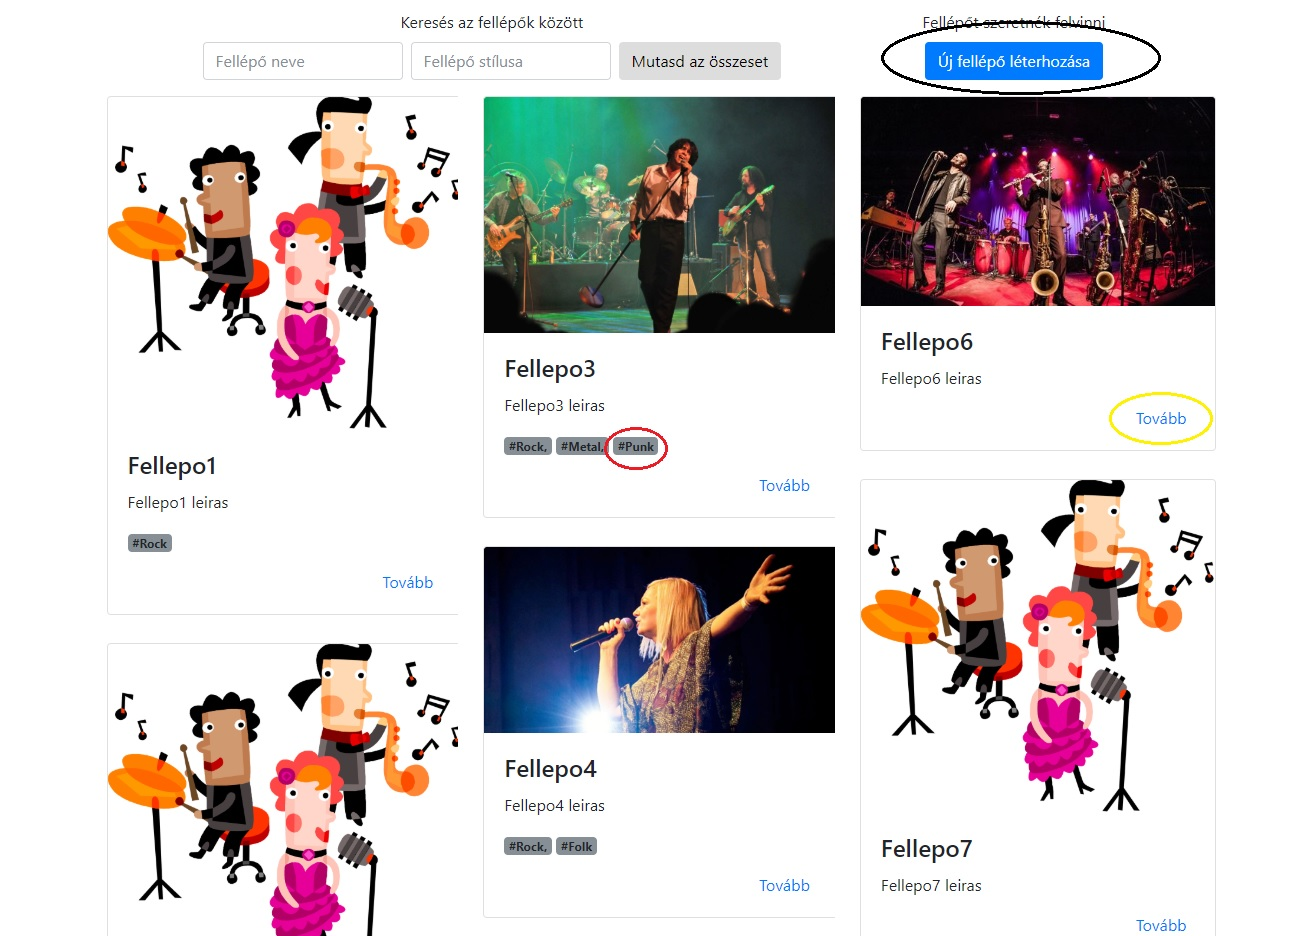
\includegraphics[scale=0.45]{kepek/artistList.jpg}
\caption{Fellépők listája}
\label{fig:artistList}
\end{figure}

Kezdjük a fellépők listázásával, a navbar-on a fellépőkre kattintással az \ref{fig:artistList} ábrán látható kép fogad bennünket. Amint látható, kilistázza a program az összes fellépőt ami le van tárolva benne. Amelyikhez van kép is elmentve, ahhoz a képet is betölti, amelyikhez nincs ahhoz pedig egy alapértelmezett képet rendel. A  két keresőmezőbe, ha beleírunk valami szöveget akkor leszűri azokra, amelyek tartalmazzák a beírt szövegrészletet értelemszerűen a fellépő nevénél a nevére, a stílusnál a stílusra szűr. Jobb felül a kék gomb amit be is karikáztam, az csak akkor jelenik meg, ha a felhasználó bejelentkezik, és ahogy a felírata is mutatja új fellépő  rögzítési helyéhez navigál. A stílusra kattintásra leszűri az olyan stílusuakra a halmazt, mint amire kattintottunk, ezt bordóval jelöltem. A továbbra kattintva a  fellépő részleteit ismerhetjük meg.

\begin{figure}
\centering
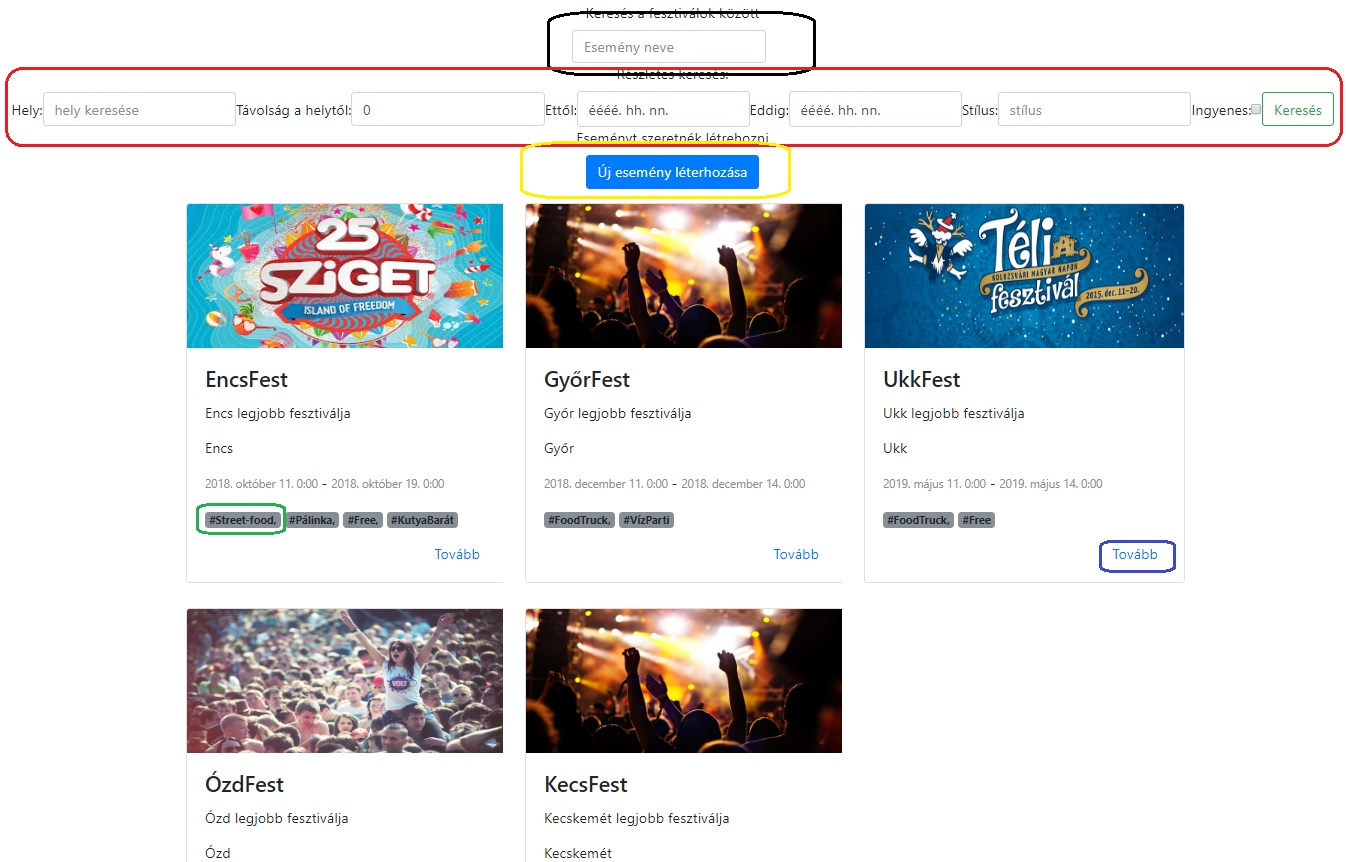
\includegraphics[scale=0.45]{kepek/festList.jpg}
\caption{Fesztiválok listája}
\label{fig:festList}
\end{figure}

Az első keresés az hasonló lesz mint a fellépők listázásánál, viszont itt csak névre lehet a gombnélküli direktszűrő funkciót alkalmazni. A részletes keresés részt már kitárgyaltuk részletesen, ezt a funkciót a következő (piros blokkban) láthatjuk az \ref{fig:festList} ábrán. Sajnos nem nagyon értek a dízájnhoz, így kicsit összecsúsztak, de funkcióját tekintve működik. A többi dolog úgy működik, mint a fellépők listázásánál.

\begin{figure}
\centering
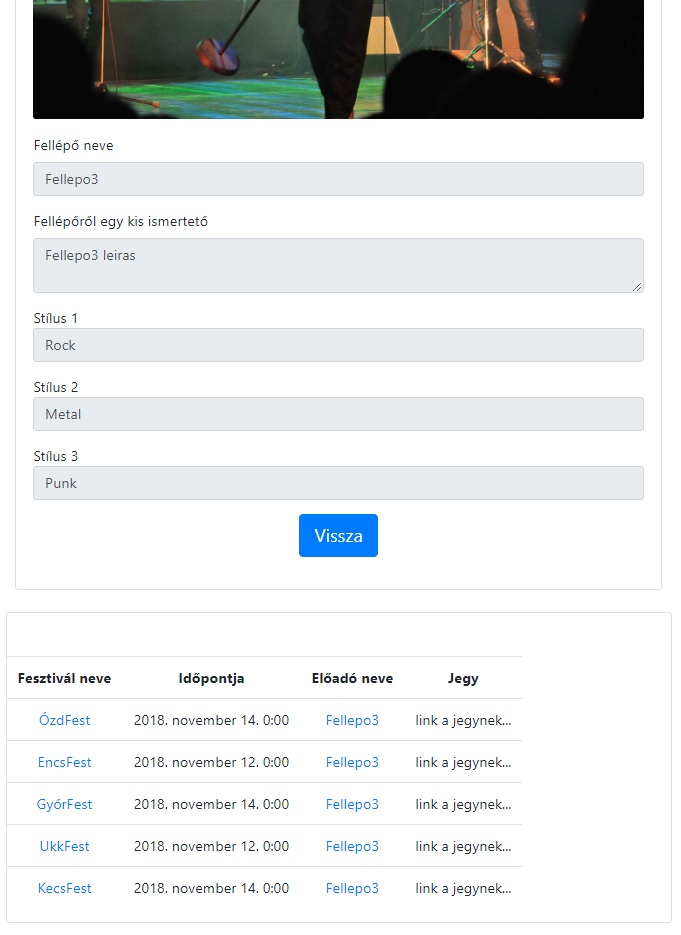
\includegraphics[scale=0.8]{kepek/artistDet.jpg}
\caption{Fellépők részletei}
\label{fig:artistDet}
\end{figure}

Fellépő részletei, amint az \ref{fig:artistDet} ábrán látható itt nem aktívak az input mezők, mert nem vagyunk belépve, ha belépünk akkor megjelenik egy szerkesztés gomb és ha arra kattintunk akkor szerkeszthetjük az adatokat. Ezt meglehetett volna úgy is oldani, hogy nem input mezőbe vezetem ki a tulajdonságokat, hanem egy külön nézetet készítek a szerkesztésnek és a nem szerkesztési résznek és nem csak a szerkeszthetőségét tiltom le. Az alsó részen a fellépő koncert naptárát tekinthetjük meg.

\begin{figure}
\centering
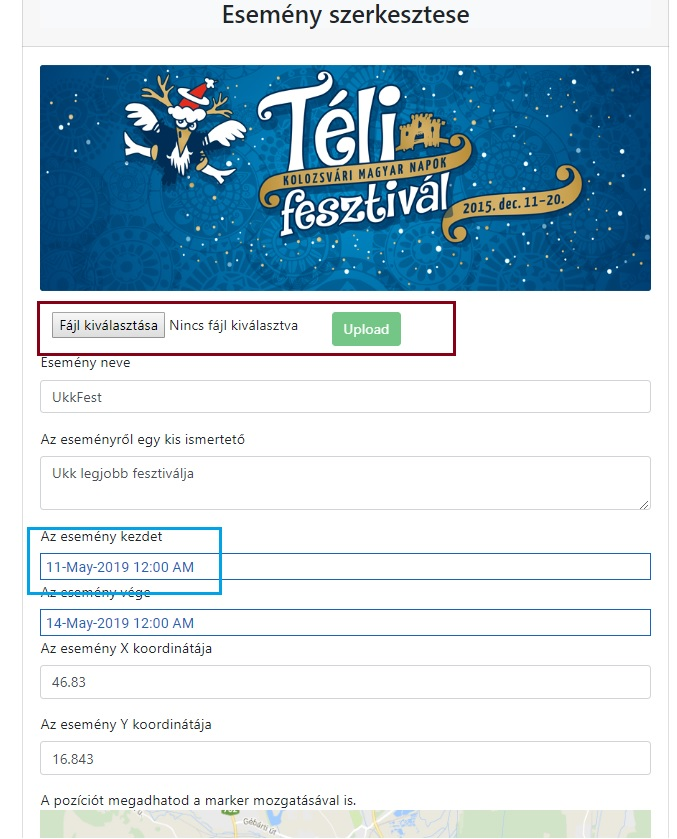
\includegraphics[scale=0.8]{kepek/eventDet.jpg}
\caption{Fesztiválok részletei}
\label{fig:event1Det}
\end{figure}

Esemény részletei, itt egy belépett felhasználó esetén láthatjuk aki rá kattintott a szerkesztés gombra. A fesztivál képe alatt ilyenkor megjeleni a képfeltöltő blokk, ha kiválasztunk egy képet feltöltésre, akkor az upload gombra kattintva tölthetjük fel. Az esemény kezdete és vége egy Date-Time-Picker segítségével választható ki, ezt majd később meg is mutatom kinyitott állapotban.  Az esemény koordinátáit lehet kézzel szerkeszteni vagy a térképen levő marker(fekete oválisban lévő píros tüske) segítségével, ezt a markert csak szerkesztés módban lehet mozgatni.  A lilával jelölt körben lévő X segítségével törölhetjük a stílusokat, illetve a narancs sárga oválisban található feliratra kattintva újat hozhatunk létre. A mentéssel rögzíthetjük a változásokat, új fesztivál felvitele esetén csak szimplán lementjük új fesztiválként, ebből leszűrhetó az is, hogy ugyanezt az űrlapot töltjük be új felvitele esetén is. A törlésre kattintva törölhetjük a fesztivált az adatbázisból. 

\begin{figure}
\centering
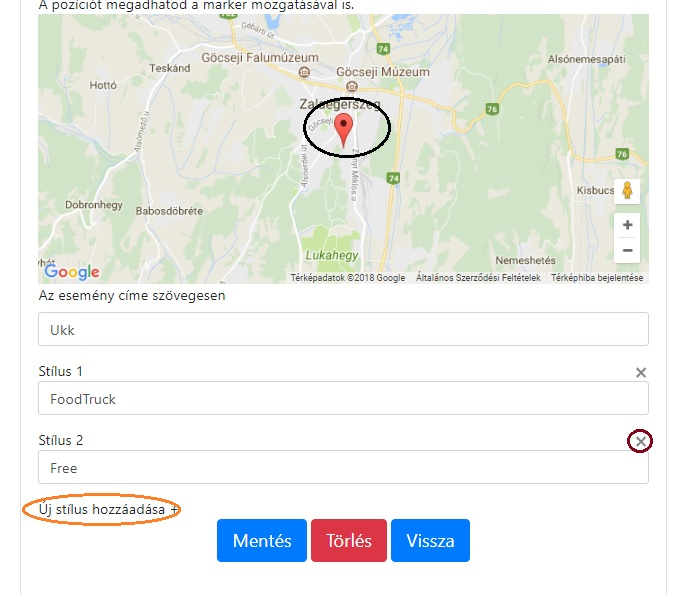
\includegraphics[scale=0.64]{kepek/eventDet2.jpg}
\caption{Fesztiválok részletei}
\label{fig:event2Det}
\end{figure}
A következő blokkban találjuk a fesztivál programját. Itt a fesztivál nevére kattintva elnavigálhatunk a fesztiválhoz, de ez az eset főleg a fellépőknél érdekes. Az előadó nevére kattintva pedig az előadó részleteit tekinthetjük meg. Az utolsó részben pedig szállásokat ajánlunk a fesztiválozók számára, ezek a fesztiváltól maximum 5 km-re elhelyezkedő szállások lesznek. A tovább gombra kattintva elnavigáljuk a fesztivál weboldalára. 
\begin{figure}
\centering
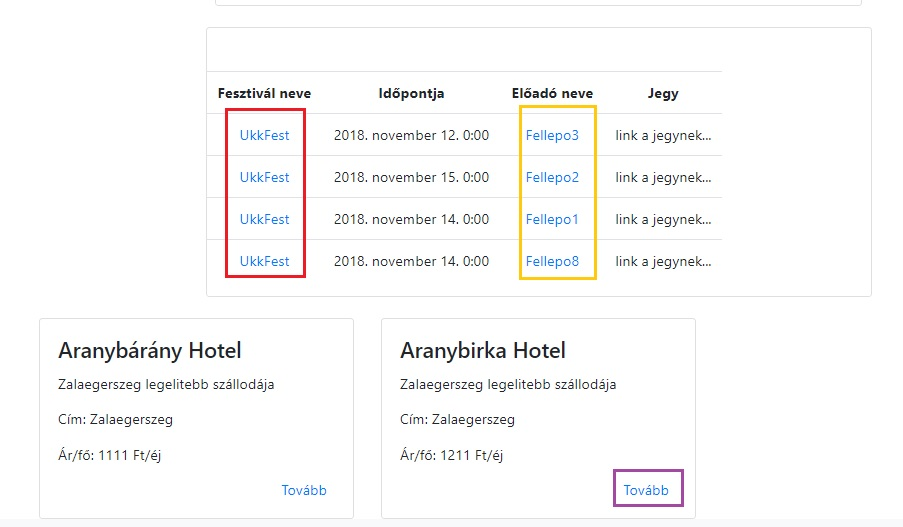
\includegraphics[scale=0.64]{kepek/festFoot.jpg}
\caption{Fesztiválok részletei}
\label{fig:event3Det}
\end{figure}
Az oldal fejlécét találjuk, itt találjuk a menüket, amik közül lehet választani. Az eseményekre kattintva jönnek be a fesztiválok listája, a fellépőkre kattintva a fellépők listája. Az új szállás és az új koncert menü csak akkor jelenik meg a nav-bar-on, ha bejelentkezünk. A profile-ra írányít bennünket az oldal ha sikerült belépnünk. A kilépéssel hagyhatjuk el az oldalt. Amég nem lépünk be addig az utolsó négy menű nem látszik, viszont van helyette bejelentkezés és regisztráció fül. A sárgával jelölt részen látható nyilak jelzik, hogy ez egy lenyilló lista. A listaelemek pedig a fesztiválok és a fellépők. A koncert időpontját itt is picker segítségével választhatjuk ki.  
\begin{figure}
\centering
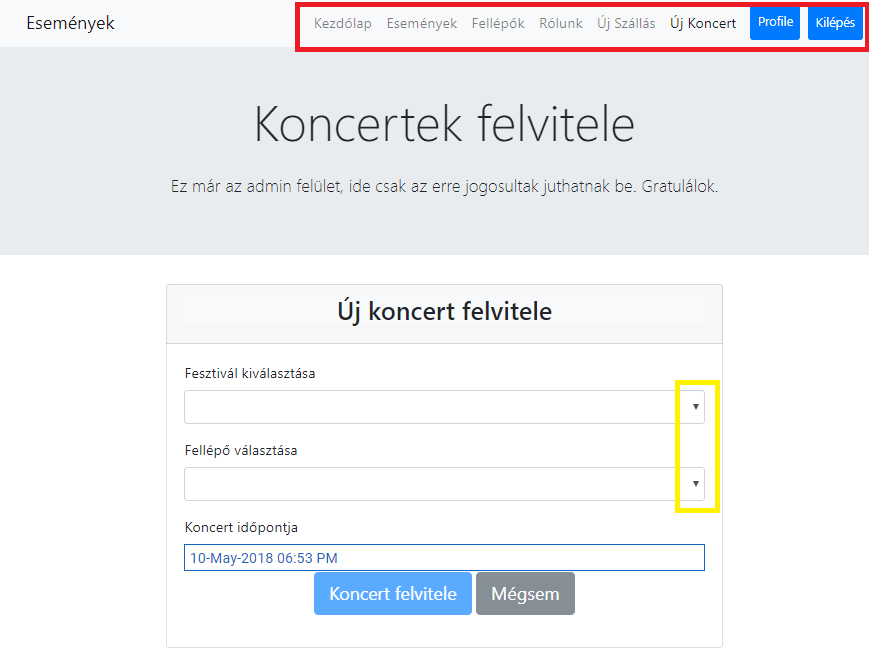
\includegraphics[scale=0.64]{kepek/concertUp.png}
\caption{Koncert rögzítése}
\label{fig:concert}
\end{figure}
A fesztivál listát láthatjuk kinyítva és a pickert. A fesztiválok listájában csak a még el nem múlott fesztiválok jelennek meg. A date-time-picker segítségével pedig könnyedén kiválaszthatjuk a számunkra kellő dátumot.
\begin{figure}
\centering
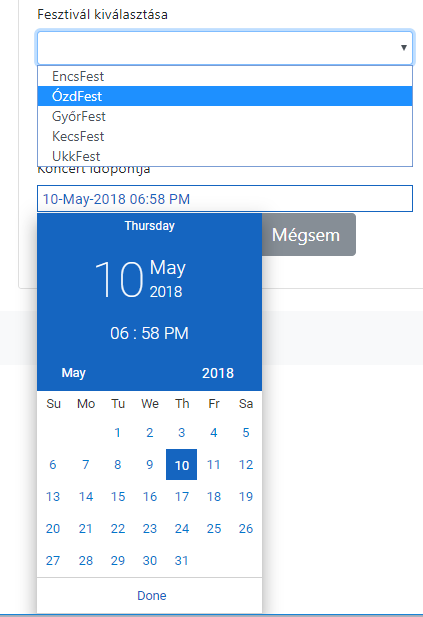
\includegraphics[scale=0.64]{kepek/concertUpOpen.png}
\caption{Koncert rögzítése}
\label{fig:concertOpen}
\end{figure}